\subsection{Requisito 1}
    \label{subsec:result_req1}
Devido à pouca fluência sobre a biblioteca~\emph{NumPy} este foi o requisito mais desafiador, já que a abordagem de manipulação das imagens comumente utilizada nas linguagens C/C++ foi utilizada: uso de laços~\emph{for}, o que tem baixíssima performance em Python.

Uma vez utilizando a biblioteca, os algoritmos foram avaliados tanto no original quanto normalizados, com exceção da~\emph{Janela Deslizante Adaptativa} por ser um algoritmo de baixa performance temporal. A Tabela~\ref{tab:result_req1_perf} traz os desempenhos sobre os dados originais, encontrando os melhores resultados para ambas as imagens base com a~\emph{Janela Deslizante} de tamanho $15$ e os piores com a~\emph{OpenCV} independente do tamanho da janela. Para os dados normalizados, a Tabela~\ref{tab:result_req1_perf_norm}, encontrando os melhores resultados para ambas as imagens com a~\emph{OpenCV} variando o tamanho entre $9-11$ e os piores com a~\emph{Busca Linear} para ``Jadeplant'' e com a~\emph{Correlação Cruzada} para ``Playtable'' ambas com janelas de tamanho $5$.

\begin{table}[!ht]
    \centering
    \small
    \begin{tabular}{c|c|c|c|c|c|c|c|c}
        \cline{3-9}
        \multicolumn{2}{l}{} & \multicolumn{7}{c}{Tamanho do bloco, $N$} \\ \hline
        Algoritmo & Imagem & 3 & 5 & 7 & 9 & 11 & 13 & 15 \\ \hline
        \multirow{2}{*}{OCV} & Jadeplant & \textcolor{violet}{$0.0$} & $0.0$ & $0.0$ & $0.0$ & $0.0$ & $0.0$ & $0.0$ \\ \cline{2-9}
         & Playtable & \textcolor{violet}{$0.0$} & $0.0$ & $0.0$ & $0.0$ & $0.0$ & $0.0$ & $0.0$ \\ \hline
        \multirow{2}{*}{BL} & Jadeplant & $0.62$ & $0.81$ & $0.72$ & $0.88$ & $1.41$ & $0.59$ & $0.55$ \\ \cline{2-9}
         & Playtable & $1.84$ & $0.75$ & $0.78$ & $1.53$ & $1.37$ & $1.46$ & $1.39$ \\ \hline
        \multirow{2}{*}{CC} & Jadeplant & $1.01$ & $1.08$ & $0.95$ & $0.9$ & $0.89$ & $0.88$ & $0.86$ \\ \cline{2-9}
         & Playtable & $3.41$ & $5$ & $1.32$ & $0.93$ & $0.79$ & $0.72$ & $0.68$ \\ \hline
        \multirow{2}{*}{JD} & Jadeplant & $2.33$ & $3.29$ & $4.18$ & $5.04$ & $5.89$ & $6.74$ & \textcolor{teal}{$7.56$} \\ \cline{2-9}
         & Playtable & $31.56$ & $40.74$ & $45.12$ & $47.84$ & $49.55$ & $50.76$ & \textcolor{teal}{$51.66$} \\ \hline
        \multirow{2}{*}{JDA} & Jadeplant & - & $2.62$ & - & - & - & - & - \\ \cline{2-9}
         & Playtable & - & - & - & - & - & - & - \\ \hline
    \end{tabular}
    \caption{Desempenho percentual dos acertos dos algoritmos com base na métrica BAD2.0.}
    \label{tab:result_req1_perf}
\end{table}

\begin{table}[!ht]
    \centering
    \small
    \begin{tabular}{c|c|c|c|c|c|c|c|c}
        \cline{3-9}
        \multicolumn{2}{l}{} & \multicolumn{7}{c}{Tamanho do bloco, $N$} \\ \hline
        Algoritmo & Imagem & 3 & 5 & 7 & 9 & 11 & 13 & 15 \\ \hline
        \multirow{2}{*}{OCV} & Jadeplant & $8.47$ & $9.15$ & $12.47$ & $46.66$ & \textcolor{teal}{$52.13$} & $51.31$ & $50.22$ \\ \cline{2-9}
         & Playtable & $4.65$ & $4.66$ & $4.68$ & \textcolor{teal}{$55.85$} & $54.92$ & $54.85$ & $53.77$ \\ \hline
        \multirow{2}{*}{BL} & Jadeplant & $4.47$ & $4.09$ & $3.93$ & $4.04$ & $4.12$ & $4.25$ & $4.36$ \\ \cline{2-9}
         & Playtable & $4.53$ & \textcolor{violet}{$4.05$} & $4.13$ & $5.25$ & $5.11$ & $4.87$ & $4.75$ \\ \hline
        \multirow{2}{*}{CC} & Jadeplant & $3.75$ & \textcolor{violet}{$3.64$} & $3.7$ & $3.82$ & $3.9$ & $3.93$ & $3.98$ \\ \cline{2-9}
         & Playtable & $5.29$ & $8.86$ & $17.3$ & $29.53$ & $38.64$ & $39.47$ & $36.86$ \\ \hline
        \multirow{2}{*}{JD} & Jadeplant & $4.13$ & $4.07$ & $4.04$ & $4$ & $3.97$ & $3.95$ & $3.94$ \\ \cline{2-9}
         & Playtable & $8.07$ & $7.68$ & $7.71$ & $7.76$ & $7.84$ & $7.91$ & $7.96$ \\ \hline
        \multirow{2}{*}{JDA} & Jadeplant & - & - & - & - & - & - & - \\ \cline{2-9}
         & Playtable & - & - & - & - & - & - & - \\ \hline
    \end{tabular}
    \caption{Desempenho percentual dos acertos dos algoritmos normalizados com base na métrica BAD2.0.}
    \label{tab:result_req1_perf_norm}
\end{table}

A partir da Figura~\ref{fig:result_req1_disp_map} fica claro o motivo da~\emph{OpenCV} ficar com os piores resultados: os valores ficaram em um~\emph{range} muito superior ao esperado ($[-30000, 10000]$ frente ao $[27, 600]$, para a ``Jadeplant'' e $[0, 4000+]$ frente ao $[27, 270]$, para a ``Playtable''); o mesmo não pode ser dito sobre os melhores. Para estes últimos, a grande quantidade de detalhes da ``Jadeplant'' não foi bem administrada pelos algoritmos, uma vez que nenhum teve um aproveitamento acima de $10\%$, mas como a ``Playtable'' possui regiões mais constantes os algoritmos tiveram melhores desempenhos. Ao passo que ao normalizar os resultados no~\emph{range} $[0, 255]$, como ilustrados na Figura~\ref{fig:result_req1_disp_map_norm}, o algoritmo da~\emph{OpenCV} detêm os melhores resultados por possuir os blocos correspondentes mais bem definidos e na mesma faixa do~\emph{groun truth} normalizado.

\begin{figure}[!ht]
    \centering
    \begin{tabular}{cc}
        \bmvaHangBox{\fbox{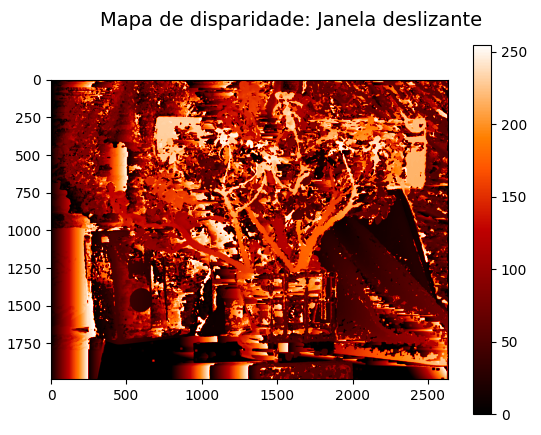
\includegraphics[width=5cm]{Figs/Resultados/jd_windowing_disp_map_bl15.png}}}&
        \bmvaHangBox{\fbox{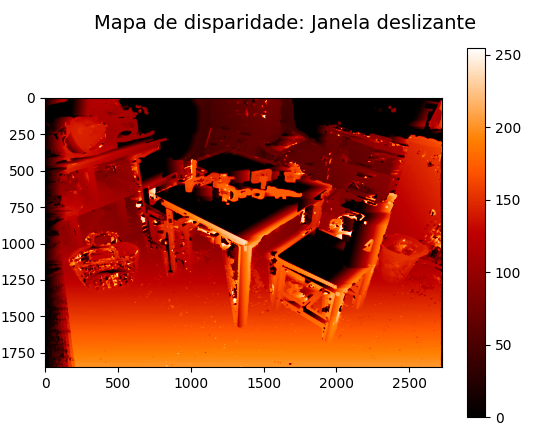
\includegraphics[width=5cm]{Figs/Resultados/pt_windowing_disp_map_bl15.png}}}\\
        (a)&(b) \\
        \bmvaHangBox{\fbox{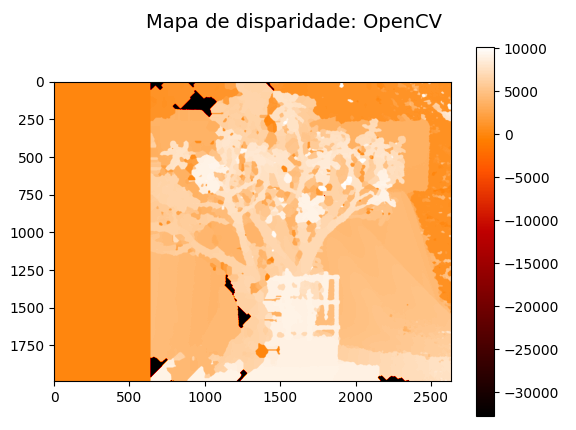
\includegraphics[width=5cm]{Figs/Resultados/jd_basic_disp_map_bl3.png}}}&
        \bmvaHangBox{\fbox{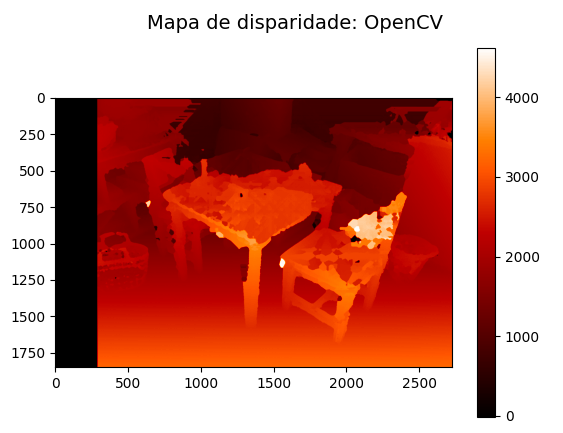
\includegraphics[width=5cm]{Figs/Resultados/pt_basic_disp_map_bl3.png}}}\\
        (c)&(d)
    \end{tabular}
    \caption{Mapas de disparidade dos melhores e piores resultados, onde (a) e (c) são o melhor e o pior, respectivamente, para ``Jadeplant'' e (b) e (d) para ``Playtable''.}
    \label{fig:result_req1_disp_map}
\end{figure}

\begin{figure}[!ht]
    \centering
    \begin{tabular}{cc}
        \bmvaHangBox{\fbox{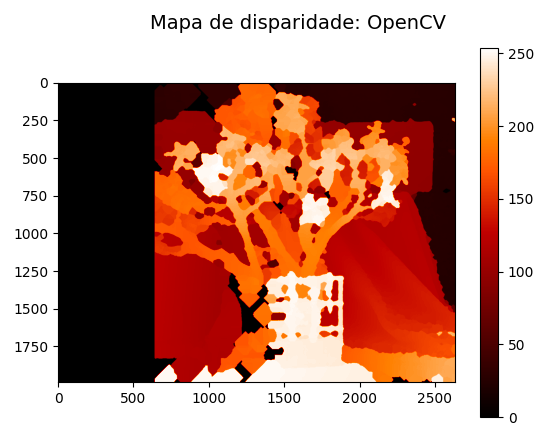
\includegraphics[width=5cm]{Figs/Resultados/eq_jd_basic_disp_map_bl11.png}}}&
        \bmvaHangBox{\fbox{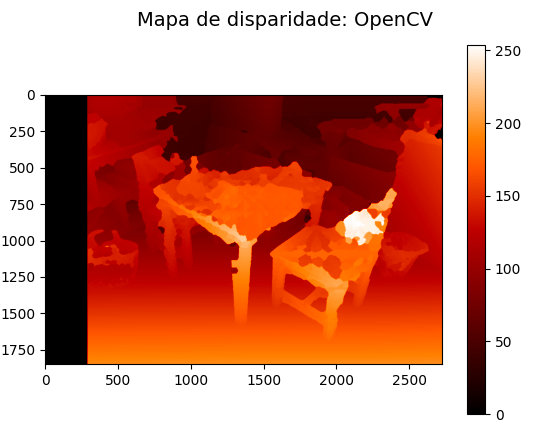
\includegraphics[width=5cm]{Figs/Resultados/eq_pt_basic_disp_map_bl9.png}}}\\
        (a)&(b) \\
        \bmvaHangBox{\fbox{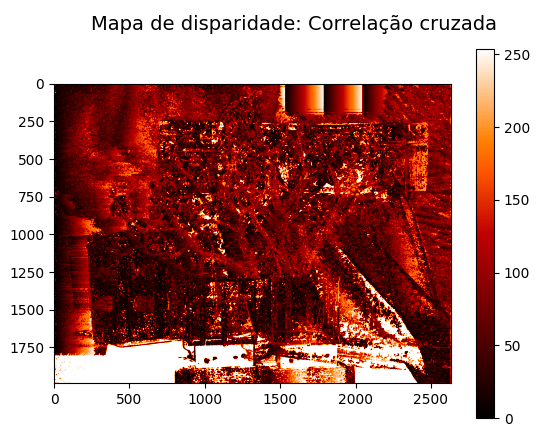
\includegraphics[width=5cm]{Figs/Resultados/eq_jd_x_correlation_disp_map_bl5.png}}}&
        \bmvaHangBox{\fbox{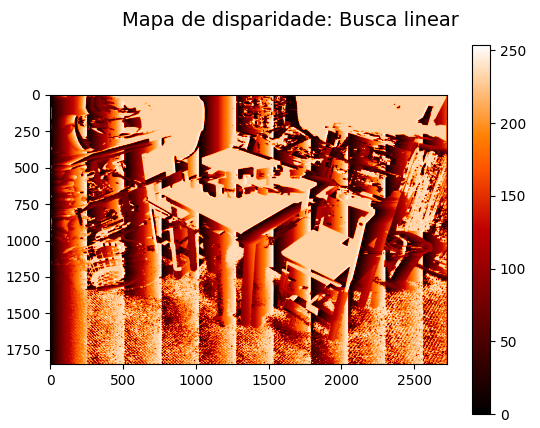
\includegraphics[width=5cm]{Figs/Resultados/eq_pt_linear_search_disp_map_bl5.png}}}\\
        (c)&(d)
    \end{tabular}
    \caption{Mapas de disparidade normalizados dos melhores e piores resultados, onde (a) e (c) são o melhor e o pior, respectivamente, para ``Jadeplant'' e (b) e (d) para ``Playtable''.}
    \label{fig:result_req1_disp_map_norm}
\end{figure}

Na análise sobre os mapas de profundidade, os erros nos cálculos dos mapas de disparidade tornam-se mais evidentes, já que a Figura~\ref{fig:result_req1_depth_map} demonstram-os como imagens de valor único e de baixíssima profundidade, ou seja, simplesmente errados. Com base nos dados das câmeras, a variação de profundidade deveria estar entre $4,63$ ($d_{xy}=600$) e $102,99$ ($d_{xy}=27$) metros para a ``Jadeplant'' e entre $1,67$ ($d_{xy}=270$) e $16,65$ ($d_{xy}=27$) para a ``Playtable''.

\begin{figure}[!ht]
    \centering
    \begin{tabular}{cc}
        \bmvaHangBox{\fbox{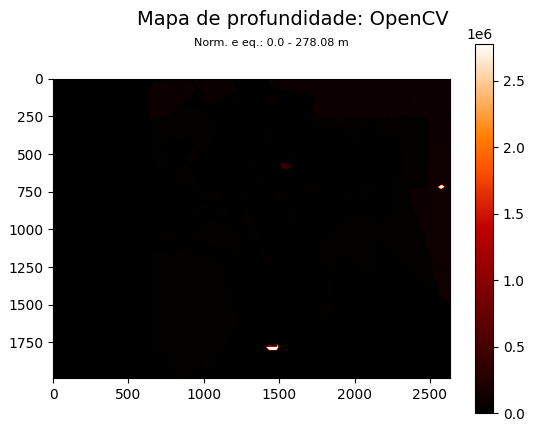
\includegraphics[height=4.5cm]{Figs/Resultados/eq_jd_dp_basic_disp_map_eq_bl11.png}}}&
        \bmvaHangBox{\fbox{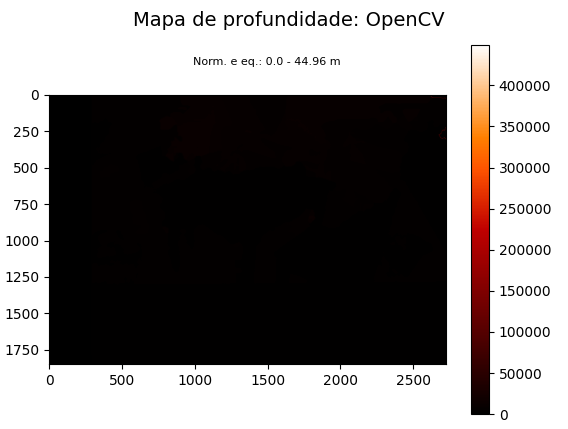
\includegraphics[height=4.5cm]{Figs/Resultados/eq_pt_dp_basic_disp_map_eq_bl9.png}}}\\
        (a)&(b)
    \end{tabular}
    \caption{Mapas de profundidade para os mapas de disparidade com as melhores taxas de acertos, onde (a) é o melhor para a ``Jadeplant'' e (b) para ``Playtable''.}
    \label{fig:result_req1_depth_map}
\end{figure}